\documentclass[11pt]{article}
\usepackage[margin=1in]{geometry}
\usepackage{amsmath,amssymb,amsthm}
\usepackage{booktabs,array}
\usepackage{graphicx}
\usepackage{float}
\usepackage{xcolor}
\usepackage{tikz}
\usetikzlibrary{positioning,calc}
\usepackage[hidelinks]{hyperref}
\usepackage{xurl}
\hypersetup{pdftitle={Supplementary Material - A Decision-Diagnostic Framework for Incomplete Machine Learning Leaderboards: Evidence Ambiguity versus Certificate Failure under Task Reweighting},pdfauthor={Ghassan Malkawi; Ahmed Elsayed; Mohammed Alhagyan; Bakeel Hussein}}
\usepackage{fontspec}
\setlength{\emergencystretch}{3em}
\renewcommand{\thefigure}{S\arabic{figure}}
\renewcommand{\thetable}{S\arabic{table}}
\renewcommand{\theequation}{S\arabic{equation}}

\title{Supplementary Material\\A Decision-Diagnostic Framework for Incomplete Machine Learning Leaderboards: Evidence Ambiguity versus Certificate Failure under Task Reweighting}
\author{Ghassan Malkawi \and Ahmed Elsayed \and Mohammed Alhagyan \and Bakeel Hussein}
\date{Corresponding author: Ghassan Malkawi (gmalkawi@hct.ac.ae)}

\begin{document}
\maketitle

\section*{S1. Purpose and scope}
This supplement provides the technical and reproducibility detail that supports the main manuscript without duplicating its narrative. The main paper states the research question, theorem claims, real-data findings, and practical interpretation. The supplement records the quantifier structure, verification scope, study design, numerical checks, and claim boundaries.

\section*{S2. Decision quantifiers and notation}
For task $d\in\{1,\ldots,D\}$, method $m\in\{1,\ldots,M\}$, and fold $k\in\{1,\ldots,N_d\}$, $x_{dkm}$ is the lower-is-better loss. A disclosure transcript $h$ fixes the fold vectors already observed. The completion set $\mathcal X(h)$ contains every complete loss array that agrees with those observations and with the declared score domains.

Within each task, methods are mapped to normalized midranks $R_{dm}\in[0,1]$, with $0$ best, $1$ worst, and exact ties receiving the same midrank. For candidate and rival indices $i,j\in\{1,\ldots,M\}$ with $j\neq i$, and admissible task weights $w$, the weighted rank gap $G_{ij}(X,w)$ is positive exactly when $j$ defeats $i$.

The total-variation neighborhood $\mathcal W(p,\varepsilon)$ contains nonnegative task weights that sum to one and satisfy $\tfrac12\lVert w-p\rVert_1\le \varepsilon$, where $\lVert\cdot\rVert_1$ is the $\ell_1$ norm. Thus $\varepsilon$ measures redistributed task-weight mass. It is not a probability, confidence level, or perturbation of model scores.

For a complete benchmark $X$, candidate $i$ is a common weak winner when $G_{ij}(X,w)\le 0$ for every admissible $w$ and every rival $j$. Under partial evidence, ``no common weak winner'' is semantically determined when every compatible completion excludes every candidate, while the defeating weight and rival may vary with the completion.

An explicit pair of compatible completions with opposite decision labels proves an information-limited state. A certificate-limited state requires a separate proof that the decision is fixed over all compatible completions together with a proof that no valid certificate exists in the declared family. Failure of an incomplete certificate search alone is inconclusive. If neither information limitation nor semantic determination is established, the state is also reported as inconclusive. The restricted certificate studied in the paper selects, for each candidate, one probability distribution over admissible weight/rival actions that must have positive expected defeat gap for every compatible completion; the theorems show that this restriction can be incomplete.

\section*{S3. Exact four-task obstruction}
The nonuniform construction uses four methods labeled A--D and four tasks, nominal task weights $p=(21,21,21,5)/68$, and $\varepsilon=13/400$. One task is partially observed and three are fully observed. All raw losses lie in $[0,1]$, aggregation is the exact arithmetic mean, and ties use exact normalized midranks.

The uncertain task admits six feasible normalized-rank patterns. The analytical argument establishes that every compatible completion has no common weak winner. Separately, two legal completions are sufficient to obstruct every completion-independent fixed joint mixture for candidate A by convexity. This establishes incompleteness of the specified certificate family.

The verification materials for the four-task construction include exact evidence JSON with SHA-256 \url{8d96a68de17e5bb02966458dd4a17d6063f679df3a5040b6dbe93cd501fc4d8f} and machine-audit JSON with SHA-256 \url{c718d5bea6a8ddb36a4af78e57f6c1eddae05d2ef291e3bf67dff11b6dc71183}.

\subsection*{S3.1 Detailed proof of the four-task obstruction}
For the uncertain task, write the normalized ranks of B, C, and D as $(r_B,r_C,r_D)$ while A has rank 1. The six feasible triples are given in Equation~\eqref{eq:s_types}:
\begin{equation}\label{eq:s_types}
(0,\tfrac13,\tfrac23),\;(\tfrac13,0,\tfrac23),\;(\tfrac16,\tfrac16,\tfrac23),\;(0,\tfrac12,\tfrac12),\;(\tfrac12,0,\tfrac12),\;(\tfrac13,\tfrac13,\tfrac13).
\end{equation}
All are realizable by the declared closed mean intervals. In every row, $r_B+r_C+r_D=1$ and $r_D\ge 1/3$.

To exclude A in every completion at the nominal weights, define $g=(1-r_B,1-r_C,1-r_D)$ and $t=(5/6,2/3,1/2)$. The three A-minus-rival nominal gaps are
\begin{equation}\label{eq:s_vj}
v_j=\frac{21}{68}(g_j-t_j)-\frac{5}{102}.
\end{equation}
Both $g$ and $t$ sum to 2, but $t$ is not one of the feasible $g$ vectors and all feasible coordinates lie on the $1/6$ lattice. Hence some coordinate satisfies $g_j-t_j\ge 1/6$, which gives
\begin{equation}\label{eq:s_A_margin}
\max_j v_j\ge \frac{21}{68\cdot6}-\frac{5}{102}=\frac1{408}>0.
\end{equation}
Thus A is excluded in every legal completion.

Each of B, C, and D is excluded by a feasible TV transfer of mass $\varepsilon=13/400$. The largest possible A-minus-rival gaps after the stated transfers are, respectively,
\begin{equation}\label{eq:s_nonA_gaps}
-\frac{211}{4080},\qquad -\frac{1}{4080},\qquad -\frac{211}{4080},
\end{equation}
so every non-A candidate is strictly defeated by A somewhere in the admissible TV neighborhood. This establishes that every compatible completion has no common weak winner.

To show that no completion-independent joint mixture can uniformly exclude A, consider the two legal uncertain-task mean rows $z_1=(3/4,0,1/8,1/4)$ and $z_2=(3/4,1/4,1/4,1/4)$. On the arithmetic average of their rank tables, the maximum A-minus-rival supports over the TV neighborhood are
\begin{equation}\label{eq:s_convex_supports}
-\frac{11}{40800},\qquad -\frac{29}{5100},\qquad -\frac{11}{40800}
\end{equation}
for B, C, and D. For any fixed probability mixture $\mu$ over admissible $(w,j)$ actions, linearity of the payoff in the rank table therefore implies
\begin{equation}\label{eq:s_mixture}
\frac{F_\mu(z_1)+F_\mu(z_2)}2<0.
\end{equation}
At least one of the two legal completions must consequently have $F_\mu(z)<0$. Hence no fixed completion-independent mixture succeeds on every compatible completion, even though the semantic no-common-weak-winner decision has already been proved for every completion. The convexified average is used only in the impossibility argument; it is not assumed to be a realizable raw completion.

\section*{S4. Uniform 68-task construction}
The stronger construction uses four methods labeled A--D, 68 equally weighted tasks, and $\varepsilon=13/400$. The tasks form four blocks of sizes 21, 21, 21, and 5. The first block contains 21 independently incomplete tasks; the remaining 47 tasks are fully known. Each uncertain task can take one of six feasible rank-row types. Supplementary Figure~\ref{fig:s1_structure} visualizes this block structure and the associated symmetry reduction.

\begin{figure}[H]
\centering
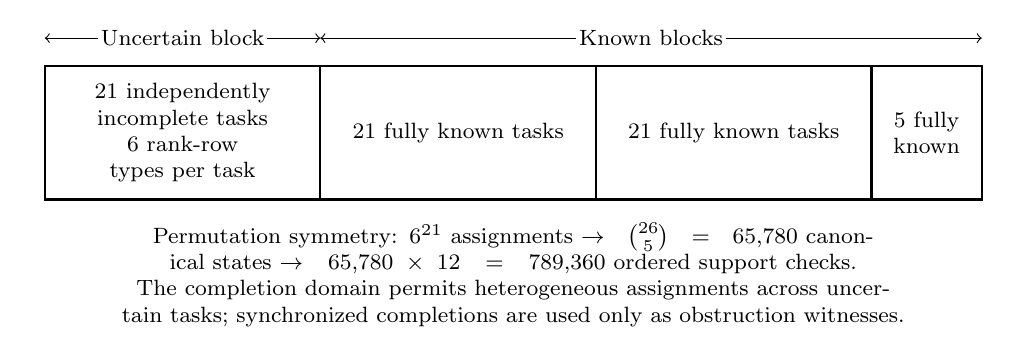
\begin{tikzpicture}[font=\footnotesize]
\def\h{1.70}
\draw[thick] (0,0) rectangle (3.5,\h);
\draw[thick] (3.5,0) rectangle (7.0,\h);
\draw[thick] (7.0,0) rectangle (10.5,\h);
\draw[thick] (10.5,0) rectangle (11.9,\h);
\node[align=center,text width=3.2cm] at (1.75,0.85) {21 independently incomplete tasks\\6 rank-row types per task};
\node[align=center,text width=3.1cm] at (5.25,0.85) {21 fully known tasks};
\node[align=center,text width=3.1cm] at (8.75,0.85) {21 fully known tasks};
\node[align=center,text width=1.2cm] at (11.2,0.85) {5 fully\\known};
\draw[<->] (0,2.05)--(3.5,2.05) node[midway,fill=white,inner sep=1pt]{Uncertain block};
\draw[<->] (3.5,2.05)--(11.9,2.05) node[midway,fill=white,inner sep=1pt]{Known blocks};
\node[align=center,text width=12.1cm] at (5.95,-0.95) {Permutation symmetry: $6^{21}$ assignments $\rightarrow \binom{26}{5}=65{,}780$ canonical states $\rightarrow 65{,}780\times12=789{,}360$ ordered support checks.\\The completion domain permits heterogeneous assignments across uncertain tasks; synchronized completions are used only as obstruction witnesses.};
\end{tikzpicture}
\caption{Structure of the 68-task uniform construction. The first 21 tasks are independently incomplete and each admits one of six feasible uncertain rank-row types. Permutation symmetry over these 21 tasks reduces the full $6^{21}$ assignment space to $\binom{26}{5}=65{,}780$ canonical states, and each state contributes 12 ordered candidate--rival support checks, yielding $789{,}360$ checks in total.}
\label{fig:s1_structure}
\end{figure}

The proof allows heterogeneous assignments across the 21 uncertain tasks. Synchronizing uncertain tasks is used only to exhibit obstruction witnesses and is not imposed on the completion domain.

Because the nominal center is uniform, permuting the 21 uncertain tasks preserves every ordered-pair support. The $6^{21}$ possible rank tables therefore reduce to the weak compositions of 21 items into six types, giving $\binom{26}{5}=65{,}780$ canonical states.

The independent exact checker evaluates 12 ordered candidate--rival comparisons for each canonical state:
\begin{equation}\label{eq:s_checks}
65{,}780\times 12 = 789{,}360\text{ ordered support comparisons.}
\end{equation}
All 63 nonempty subsets of the six uncertain row types were also checked in the verification archive. Exact integer transport and a separate rational-arithmetic implementation agree on the support signs. A fresh replay from the archived verification materials on Python 3.13.5 reproduced the same verification outcome obtained previously on Python 3.12.14.

The archived uniform-construction verification artifact used in that replay has SHA-256: \url{ca61a164846342f5489cbbf3c9f068b3d1d76e8314ff549f46288b57de6fcd50}.

\section*{S5. Real TabArena study design}
The empirical study uses real benchmark evidence from TabArena. The study data contain 51 tasks, 14 prespecified methods, and 816 paired fold vectors. One disclosure reveals the complete method-loss vector for one recorded fold of one task.

The study fixes the task set, candidate set, score direction, fold aggregation, normalized-midrank rule, nominal task weights, TV radius, and numerical target before screening prefixes. The 80 traces are generated by four declared disclosure policies, ten seeds, and two radii, $\varepsilon=2/51$ and $\varepsilon=4/51$. The traces share the same benchmark archive.

Across 480 prespecified checkpoints, the tested mixed-rival strengthening produced no earlier stopping than the recorded stopping status.

\section*{S6. Opposite-answer completion witnesses}
For each trace, let $Q$ be the recorded stopping disclosure count. The information-limitation analysis examines its immediate predecessor $q=Q-1$. A successful witness consists of two legal complete arrays that agree on every disclosed fold vector but have opposite values of the decision predicate defined in the main paper.

The archived completion supplies one label. Constructed completions use only the disclosed observations and declared score domains; the actual unseen fold values and actual unseen decision label are not inputs to the construction.

The initial constant-fill recipe supplied witnesses on 36 of 80 traces. A second prespecified equalization-based recipe retained all 36 and raised the total to 47. The second rule evaluated 14 candidate completions per trace across all 80 traces, yielding 1,120 candidate-completion trials.

Table~\ref{tab:s1_witnesses} records the witness ledger used in the verification summary.
\begin{table}[H]
\centering
\caption{Opposite-answer witness ledger for the fixed pre-stopping prefixes.}
\label{tab:s1_witnesses}
\begin{tabular}{lrrrr}
\toprule
TV radius & Traces & Constant-fill witnesses & Proven ambiguous & Inconclusive\\
\midrule
$2/51$ & 40 & 33 & 39 & 1\\
$4/51$ & 40 & 3 & 8 & 32\\
Both & 80 & 36 & 47 & 33\\
\bottomrule
\end{tabular}
\end{table}
The 47 successful traces prove information limitation under the declared completion model. The remaining 33 traces are inconclusive.

\subsection*{S6.1 Conditional fixed-trace decision-point match}
For the same fixed disclosure order, let $h_q$ denote the first $q$ disclosed fold vectors and let $q^\star$ be the first prefix at which the decision predicate is constant over all compatible completions. A verified opposite-answer pair at $Q-1$ gives the lower bound $q^\star>Q-1$. The verified certificate at $Q$ gives the matching upper bound $q^\star\le Q$, subject to the original finite-well-defined-target scope and numerical mean-enclosure qualification. Hence all 47 successful witness traces satisfy the conditional fixed-trace match $q^\star=Q$.

Table~\ref{tab:s2_qmatch} reports these matches by disclosure policy and TV radius.
\begin{table}[H]
\centering
\caption{Conditional fixed-trace $Q$ matches by disclosure policy and TV radius. A match combines a verified ambiguity witness at $Q-1$ with the verified stopping-prefix certificate at $Q$.}
\label{tab:s2_qmatch}
\begin{tabular}{lrrr}
\toprule
Disclosure policy & TV radius & Traces & $q^\star=Q$ matches\\
\midrule
Random fold & $2/51$ & 10 & 10\\
Random fold & $4/51$ & 10 & 1\\
Random task blocks & $2/51$ & 10 & 9\\
Random task blocks & $4/51$ & 10 & 3\\
Cheapest remaining & $2/51$ & 10 & 10\\
Cheapest remaining & $4/51$ & 10 & 2\\
Decision gap & $2/51$ & 10 & 10\\
Decision gap & $4/51$ & 10 & 2\\
\midrule
Total & --- & 80 & 47\\
\bottomrule
\end{tabular}
\end{table}
The match is specific to the recorded disclosure order. It does not compare alternative query orders.

\section*{S7. Verification of real-data witnesses}
A separately implemented verifier checked agreement on disclosed values, declared score domains, mean-enclosure bounds, valid rank values, exact-tie handling, and file digests. The verification record contains 14,560 candidate support comparisons and 364 comparisons against the archived completion. Exact integer support signs determine witness acceptance; numerical linear-programming solves are diagnostic.

Because the verifier reuses the same parser and aggregation routines as the analysis, it serves as an implementation cross-check.

\section*{S8. Claim boundaries}
The claim boundaries are threefold. First, the real-data completions are logical completions under declared numerical domains and are not guaranteed to be realizable by retraining the named methods. Second, the 80 traces overlap and support no population-frequency inference. Third, the certificate obstruction applies to the specified completion-independent family, while the fixed-trace $q^\star=Q$ result applies only to the 47 witnessed traces and the recorded disclosure order.

\section*{S9. Reproducibility inventory}
Reproducibility materials are publicly available at:\\
\url{https://github.com/shaikhamalkawi-ux/decision-diagnosis-incomplete-ml-leaderboards}.\\
The public repository includes the diagnostic procedure, detailed proof materials, result summaries, verification summaries, the fixed-trace $q^\star=Q$ verifier and summary, figure-reproduction code, and provenance notes. The repository and associated verification archives include the exact-theory checker, tests, evidence, and the witness-generation and verification workflow. Third-party raw TabArena artifacts are not redistributed where redistribution rights are unclear; retrieval/provenance instructions are provided instead.

\end{document}